% =====================================================================
%  StudyBuddy - AI Study Coach Agent
%  LaTeX report (compiled on Overleaf)
%
%  Upload: Overleaf -> New Project -> Upload Project -> zip of /report
%  Screenshots go in: report/figures/
% =====================================================================
\documentclass[11pt,a4paper]{article}

\usepackage[margin=2.4cm]{geometry}
\usepackage[utf8]{inputenc}
\usepackage[T1]{fontenc}
\usepackage{lmodern}
\usepackage{graphicx}
\usepackage{xcolor}
\usepackage{booktabs}
\usepackage{enumitem}
\usepackage{listings}
\usepackage{tikz}
\usetikzlibrary{arrows.meta,positioning,shapes.geometric,fit}
\usepackage[hidelinks,linktoc=all]{hyperref}

% ---- colours ----
\definecolor{linkblue}{HTML}{2B4CD8}
\definecolor{codebg}{HTML}{F4F6FB}
\definecolor{accent}{HTML}{6C8CFF}
\definecolor{darkgrey}{HTML}{444444}
% ---- fill-in commands (edit these once) ----
\newcommand{\studentname}{FULL NAME}
\newcommand{\studentid}{STUDENT ID}
\newcommand{\coursename}{Web Client-Side Programming}
\newcommand{\instructorname}{INSTRUCTOR NAME}
\newcommand{\appurl}{https://studybuddy-XXXX.vercel.app}
\newcommand{\repourl}{https://github.com/manganjokean/studybuddy}

\hypersetup{
  colorlinks=true,
  urlcolor=linkblue,
  linkcolor=linkblue,
  pdftitle={StudyBuddy - AI Study Coach Agent},
  pdfauthor={\studentname}
}

% ---- code listing style ----
\lstset{
  basicstyle=\ttfamily\small,
  backgroundcolor=\color{codebg},
  frame=single,
  rulecolor=\color{darkgrey!40},
  breaklines=true,
  showstringspaces=false,
  columns=flexible,
  keepspaces=true,
  keywordstyle=\color{linkblue}\bfseries,
  commentstyle=\color{darkgrey},
  stringstyle=\color{darkgrey!80}
}

\setlength{\parindent}{0pt}
\setlength{\parskip}{6pt}

\begin{document}

% =====================================================================
\begin{titlepage}
  \centering
  \vspace*{1.5cm}

  {\Huge\bfseries StudyBuddy\\[6pt]\large AI Study Coach Agent\par}

  \vspace{1.2cm}
  {\Large An AI-agent web application built with Node.js, Express and the Google Gemini API\par}

  \vspace{2.2cm}

  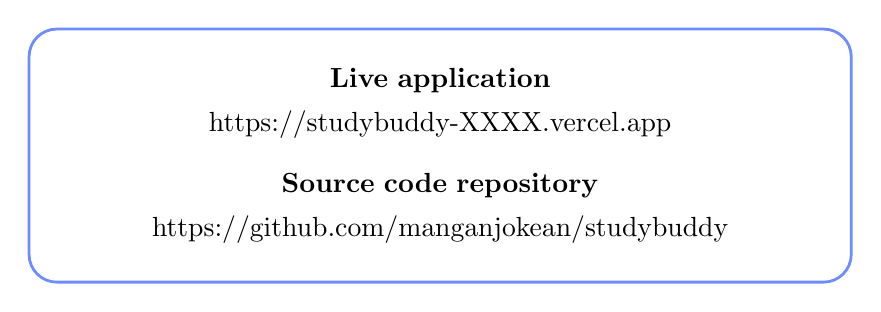
\begin{tikzpicture}
    \node[draw=accent,line width=1pt,rounded corners=10pt,inner sep=14pt,text width=0.78\textwidth,align=center]
      {
        \textbf{Live application}\\[4pt]
        \url{\appurl}\\[10pt]
        \textbf{Source code repository}\\[4pt]
        \url{\repourl}
      };
  \end{tikzpicture}

  \vfill

  {\large
    \begin{tabular}{rl}
      \textbf{Author:}      & \studentname \\[2pt]
      \textbf{Student ID:}  & \studentid \\[2pt]
      \textbf{Course:}      & \coursename \\[2pt]
      \textbf{Instructor:}  & \instructorname \\[2pt]
      \textbf{Date:}        & \today \\
    \end{tabular}\par}

  \vspace{1cm}
\end{titlepage}

% =====================================================================
\begin{abstract}
\noindent
StudyBuddy is a publicly deployed web application that helps students turn their own lecture
notes into interactive study material. The project implements an \emph{AI agent} rather than a
plain chatbot: a Node.js/Express back end exposes a set of tools to the Google Gemini model, and
an agentic loop lets the model decide which tool to call, execute it on the server, feed the
result back, and only then produce a final answer for the user. The client side is a chat
interface written in vanilla HTML, CSS and JavaScript: user and agent turns appear as bubbles, the
agent's tool calls are animated as a visible plan, and the quiz, flashcards or explanation built
by a tool are rendered inline in the same conversation.
Quiz results are persisted in the browser with \texttt{localStorage}. The application is deployed
on Vercel and the Gemini API key is kept entirely outside the repository through environment
variables, a strict \texttt{.gitignore} and an automated pre-push secret scanner.
This report describes the requirements, architecture, agent design, implementation,
deployment, security measures, testing, and lessons learned during the project.
\end{abstract}

\tableofcontents
\newpage

% =====================================================================
\section{Introduction}

Students routinely revise from passive material: re-reading slides, highlighting text and
re-reading again. Research on learning consistently favours \emph{active recall} --- retrieving
information from memory --- but producing practice questions from one's own notes is tedious.

StudyBuddy addresses this with a small, focused web application. A student pastes their notes
(or types a topic), and an AI agent decides how best to help: it can generate a quiz, build a
flashcard deck, or explain a concept at an appropriate level. The distinctive feature of the
project is that the model does not simply emit text: it \emph{calls tools} that the server
executes, and the structured output of those tools drives the interactive front end.

\subsection*{Project objectives}
\begin{itemize}[leftmargin=*]
  \item Build a working web application whose front end demonstrates client-side skills
        (DOM manipulation, \texttt{fetch}, event handling, state, local persistence, responsive CSS).
  \item Implement an AI agent with a real tool-calling loop, not a single chat completion.
  \item Deploy the application to a public host so it can be opened by anyone.
  \item Keep the API key out of source control and out of the browser.
  \item Produce this report, linked to the live application and the source repository.
  \item Present and demonstrate the application in class.
\end{itemize}

% =====================================================================
\section{Requirements}

\begin{table}[h]
\centering
\caption{Functional and non-functional requirements.}
\label{tab:reqs}
\begin{tabular}{@{}p{1.2cm}p{6.6cm}p{4.4cm}@{}}
\toprule
\textbf{ID} & \textbf{Requirement} & \textbf{Status} \\
\midrule
FR-1 & Accept study material or a free-text topic from the user & Implemented \\
FR-2 & Agent selects and executes at least two distinct tools & Implemented (3 tools) \\
FR-3 & Display the agent's plan / tool-call trace to the user & Implemented \\
FR-4 & Interactive quiz with per-question feedback and a final score & Implemented \\
FR-5 & Flashcard deck with flip interaction & Implemented \\
FR-6 & Structured concept explanation & Implemented \\
FR-7 & Persist quiz history locally in the browser & Implemented (\texttt{localStorage}) \\
FR-8 & Graceful error handling for invalid input, rate limits and API failures & Implemented \\
NFR-1 & Deployed to a public URL & Vercel \\
NFR-2 & No API key in the repository or in client-side code & Enforced by tooling \\
NFR-3 & Responsive layout, no front-end framework & Vanilla HTML/CSS/JS \\
\bottomrule
\end{tabular}
\end{table}

% =====================================================================
\section{Technology Stack}

\begin{table}[h]
\centering
\caption{Technologies used.}
\begin{tabular}{@{}llp{6cm}@{}}
\toprule
\textbf{Layer} & \textbf{Technology} & \textbf{Reason} \\
\midrule
Front end   & HTML5, CSS3, vanilla ES6 JS & Course focus: client-side programming \\
Back end    & Node.js 22+ / Express 5     & Simple static + JSON API server \\
AI model    & Google Gemini (\texttt{gemini-3.8-flash}) & Native function calling, free tier \\
API style   & REST (\texttt{generateContent}) & No SDK dependency, transparent requests \\
Hosting     & Vercel                       & Static files + Node serverless functions, free tier \\
Versioning  & Git / GitHub                 & Required repository link \\
Report      & \LaTeX~on~Overleaf & PDF output (required deliverable) \\
\bottomrule
\end{tabular}
\end{table}

% =====================================================================
\section{System Architecture}

The application is a classic two-tier structure. The browser never talks to the AI provider:
all model calls go through the back end -- an Express server during local development, a Vercel
serverless function in production -- which is the only component that holds the API key.

\begin{figure}[h]
\centering
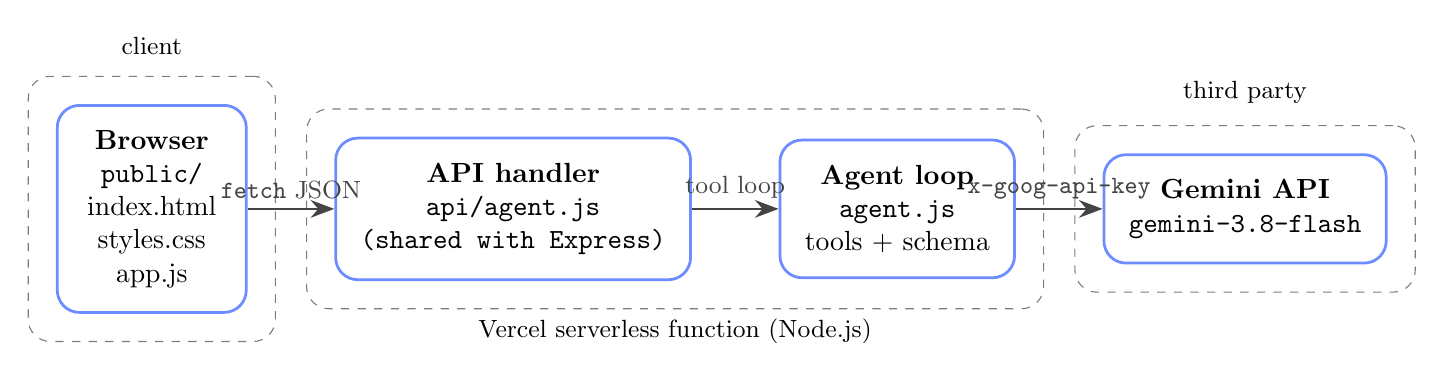
\begin{tikzpicture}[
  node distance=1.6cm and 1.1cm,
  box/.style={draw=accent, line width=1pt, rounded corners=8pt, align=center, inner sep=9pt, minimum width=2.4cm},
  host/.style={draw=darkgrey!70, dashed, rounded corners=8pt, inner sep=10pt},
  arr/.style={-{Stealth[length=3mm]}, thick, darkgrey}
]
  \node[box] (browser) {\textbf{Browser}\\ \texttt{public/}\\ index.html \\ styles.css \\ app.js};
  \node[box, right=of browser] (server) {\textbf{API handler}\\ \texttt{api/agent.js}\\ \texttt{(shared with Express)}};
  \node[box, right=of server] (agent) {\textbf{Agent loop}\\ \texttt{agent.js}\\ tools + schema};
  \node[box, right=of agent] (gemini) {\textbf{Gemini API}\\ \texttt{gemini-3.8-flash}};

  \node[host, fit=(browser)] (bhost) {};
  \node[host, fit={(server)(agent)}, label={[font=\small]below:Vercel serverless function (Node.js)}] (shost) {};
  \node[host, fit=(gemini)] (ghost) {};
  \node[font=\small, above=0.15cm of bhost] {client};
  \node[font=\small, above=0.15cm of ghost] {third party};

  \draw[arr] (browser) -- node[above,font=\small]{\texttt{fetch} JSON} (server);
  \draw[arr] (server) -- node[above,font=\small]{tool loop} (agent);
  \draw[arr] (agent) -- node[above,font=\small]{\texttt{x-goog-api-key}} (gemini);
\end{tikzpicture}
\caption{Request flow. The API key exists only inside the Vercel environment (or the developer's
local \texttt{.env}).}
\label{fig:arch}
\end{figure}

\subsection*{Project structure}
\begin{lstlisting}[language=bash]
studybuddy/
|-- server.js            # Express server for local dev, mounts ./api
|-- agent.js             # agent loop, tool schemas, tool implementations
|-- api/
|   |-- agent.js         # POST /api/agent   (Vercel function + Express route)
|   `-- health.js        # GET  /api/health  (Vercel function + Express route)
|-- vercel.json          # Vercel config: static output public/, 30s limit
|-- scripts/keycheck.js  # pre-push secret scanner
|-- scripts/shoot.mjs    # headless UI test + report screenshots
|-- public/
|   |-- index.html       # markup: chat thread, composer, artefact cards
|   |-- styles.css       # theming, quiz UI, 3D flip cards, responsive
|   `-- app.js           # fetch, trace animation, quiz logic, storage
|-- report/              # this LaTeX report + figures
|-- .env                 # API key (gitignored, never pushed)
`-- .env.example         # placeholder committed on purpose
\end{lstlisting}

% =====================================================================
\section{AI Agent Design}

\subsection*{What makes it an agent}
A chatbot performs a single request/response and returns prose. StudyBuddy's back end instead
runs a \emph{loop}:

\begin{enumerate}[leftmargin=*]
  \item The user goal, conversation history and a system prompt are sent to Gemini together with
        a list of \textbf{function declarations} (the tool schemas).
  \item If the model answers with a \texttt{functionCall}, the server executes that tool locally,
        appends a \texttt{functionResponse} containing the real result, and calls the model again.
  \item Steps repeat until the model replies with plain text, or a safety limit of four rounds is
        reached.
  \item The response returned to the browser contains three parts: the agent's natural-language
        reply, the \textbf{trace} of tools invoked, and the raw structured \textbf{results} used to
        render the interactive components.
\end{enumerate}

\begin{lstlisting}[language=Java,caption={Simplified agent loop (agent.js).}]
for (let step = 0; step < MAX_STEPS; step++) {
  const parts = await callGemini({ contents, tools: TOOLS,
                                   systemInstruction: SYSTEM_PROMPT });
  const calls = parts.filter(p => p.functionCall);
  if (!calls.length) { finalText = joinText(parts); break; }  // done

  contents.push({ role: 'model', parts });
  for (const c of calls) {
    const output = await TOOL_IMPLS[c.functionCall.name](c.functionCall.args);
    results[c.functionCall.name] = output;                    // structured result
    contents.push({ role: 'user', parts: [{ functionResponse: ... }] });
  }
}
\end{lstlisting}

\subsection*{Available tools}
\begin{table}[h]
\centering
\caption{Tools exposed to the model.}
\begin{tabular}{@{}lp{4.4cm}p{6.4cm}@{}}
\toprule
\textbf{Tool} & \textbf{Arguments} & \textbf{Behaviour} \\
\midrule
\texttt{generateQuiz} & \texttt{source, topic, count, difficulty}
  & Calls Gemini with a JSON response schema; validates each question and clamps \texttt{count} to 3--10 \\
\texttt{generateFlashcards} & \texttt{source, topic, count}
  & Produces front/back card pairs, filtered for well-formed entries \\
\texttt{explainConcept} & \texttt{concept, level}
  & Free-text answer forced into \texttt{\#\#} sections so the client can render it reliably \\
\bottomrule
\end{tabular}
\end{table}

\subsection*{Robustness measures}
\begin{itemize}[leftmargin=*]
  \item \textbf{Structured output}: quizzes and flashcards are requested as JSON with an
        explicit schema, and every returned field is validated before it reaches the browser,
        instead of trusting the model to format things correctly.
  \item \textbf{Input clamping}: question counts, string lengths and history size are bounded
        before they reach the API.
  \item \textbf{Graceful degradation}: if the final summarising call fails (for example due to a
        rate limit), the already-produced structured results are still returned with a fallback
        message, so the user is not left with an error screen.
  \item \textbf{Friendly errors}: HTTP 429, 400/403 and network failures are mapped to plain-language
        messages; technical details are written to the server log only.
\end{itemize}

% =====================================================================
\section{Client-Side Implementation}

The graded focus of the course is client-side development, so the front end is written without
any framework.

\begin{itemize}[leftmargin=*]
  \item \textbf{Conversation thread}: user and agent turns are rendered as chat bubbles with a
        typing indicator while the agent works, and the thread auto-scrolls to the newest message.
  \item \textbf{Agent trace animation}: each tool call returned by the API is appended to an
        ``Agent plan'' block one step at a time, so the audience can watch the agent decide and act
        before the answer arrives.
  \item \textbf{Inline artefact cards}: the quiz, flashcard deck or explanation produced by a tool
        is injected directly into the same conversation turn -- no page change, no separate results
        screen.
  \item \textbf{Quiz engine}: one question at a time, immediate green/red feedback together with
        the explanation, a progress pill, and a conic-gradient score ring at the end.
  \item \textbf{Flashcards}: a 3D \texttt{rotateY} flip implemented with
        \texttt{transform-style: preserve-3d} and \texttt{backface-visibility}, plus a Fisher--Yates
        shuffle.
  \item \textbf{State \& persistence}: scores are written to \texttt{localStorage} under
        \texttt{studybuddy.scores}; the last eight conversation turns are sent with every request
        so the agent can answer follow-ups in context.
  \item \textbf{Composer}: \emph{Enter} sends, \emph{Shift+Enter} inserts a newline, the textarea
        grows with its content, and mode/level/item selectors steer the agent's tool choice.
  \item \textbf{Resilience}: spinner on the send button, toast notifications for errors, and all
        dynamic text inserted through an HTML-escaping helper to avoid injection from model output.
  \item \textbf{Responsive layout}: a single-column chat shell that adapts below 780\,px, with
        touch-friendly card grids.
\end{itemize}

% ---- screenshots (export PNGs to report/figures/) ----
% Compiles even if a screenshot is missing: an empty slot is drawn instead.
\newcommand{\figslot}[1]{%
  \IfFileExists{figures/#1.png}%
    {\includegraphics[width=\linewidth]{figures/#1.png}}%
    {\fbox{\parbox[c][3.4cm][c]{0.90\linewidth}{\centering\textcolor{darkgrey}{%
      \textbf{[ screenshot pending]}\\[2pt]\texttt{figures/#1.png}}}}}}

\begin{figure}[h]
  \centering \figslot{app-welcome}
  \caption{Landing screen: capability overview, example prompts and the composer.}
  \label{fig:welcome}
\end{figure}

\begin{figure}[h]
\centering
\begin{minipage}{0.48\textwidth}
  \centering \figslot{app-main}
  \caption{Chat turn: user request, agent plan and reply.}
\end{minipage}\hfill
\begin{minipage}{0.48\textwidth}
  \centering \figslot{app-quiz}
  \caption{Inline quiz with per-question feedback.}
\end{minipage}
\end{figure}

\begin{figure}[h]
\centering
\begin{minipage}{0.48\textwidth}
  \centering \figslot{app-cards}
  \caption{Flashcard deck with flip interaction.}
\end{minipage}\hfill
\begin{minipage}{0.48\textwidth}
  \centering \figslot{app-explain}
  \caption{Structured concept explanation.}
\end{minipage}
\end{figure}

% =====================================================================
\section{Deployment}

The application is deployed on \textbf{Vercel}. Heroku, also listed in the brief, removed its free
tier; Vercel's free plan serves the static front end from \texttt{public/} and executes the API as
Node.js \emph{serverless functions}. The handlers in \texttt{api/} are \emph{the same modules} the
local Express server mounts, so local development and production run one identical code path --
only the runtime around them differs.

\begin{enumerate}[leftmargin=*]
  \item Push the repository to GitHub: \url{\repourl}.
  \item In Vercel: \emph{Add New $\rightarrow$ Project} and import the repository. The framework
        preset is \emph{Other}; \texttt{vercel.json} declares \texttt{public/} as the static
        output directory and caps each function at 30\,s.
  \item Under \emph{Settings $\rightarrow$ Environment Variables}, add \texttt{GEMINI\_API\_KEY}
        with the secret value. This is the \emph{only} place the key is stored outside the
        developer's machine.
  \item Deploy. Every push to \texttt{main} triggers a new deployment, and the site is reachable
        at \url{\appurl}.
  \item Locally, \texttt{npm start} runs the identical handlers through Express for development.
\end{enumerate}

\paragraph{Free-tier caveat.} Nothing sleeps between requests: static assets are served from a CDN
and only the two functions cold-start, which adds well under a second to the first request.
The configured 30-second function limit is comfortably above the agent's typical end-to-end
latency (three to four model calls).

% =====================================================================
\section{Security: API Key Handling}

The brief explicitly forbids pushing API keys to GitHub. This was treated as a design constraint
rather than an afterthought, and enforced at four levels:

\begin{table}[h]
\centering
\caption{Defence-in-depth for the secret.}
\begin{tabular}{@{}lp{9cm}@{}}
\toprule
\textbf{Layer} & \textbf{Mechanism} \\
\midrule
Repository   & \texttt{.gitignore} written \emph{before} the first commit; it lists \texttt{.env},
               \texttt{.env.local}, \texttt{.env.*.local} and \texttt{node\_modules/} \\
Code         & The key is read only via \texttt{process.env.GEMINI\_API\_KEY}; there is no
               fallback literal anywhere in the source \\
Transport    & The key is sent as the \texttt{x-goog-api-key} header directly to Google's API and
               is never returned in any HTTP response \\
Tooling      & \texttt{npm run keycheck} scans every text file for credential patterns
               (Google \texttt{AIza…}, OpenAI/Anthropic \texttt{sk-…}, bearer tokens, assigned key
               variables) and exits non-zero if anything matches \\
\bottomrule
\end{tabular}
\end{table}

\begin{lstlisting}[language=bash,caption={Verifying the repository before every push.}]
$ npm run keycheck
> node scripts/keycheck.js
  No API keys or secrets found in the project. Safe to push.
\end{lstlisting}

Additionally, \texttt{.env.example} is committed with placeholder values only, which documents
the required configuration without disclosing anything. The server also detects when the
placeholder was never replaced and reports \emph{``API key missing''} in the health endpoint
instead of failing obscurely at request time.

% =====================================================================
\section{Testing}

\begin{table}[h]
\centering
\caption{Test cases executed before submission.}
\begin{tabular}{@{}lp{6.4cm}l@{}}
\toprule
\textbf{Area} & \textbf{Case} & \textbf{Result} \\
\midrule
Health     & \texttt{GET /api/health} reports model and key status & Pass \\
Validation & Empty message returns \texttt{400} with a clear error & Pass \\
Validation & Oversized message rejected (\texttt{413}) & Pass \\
Errors     & Malformed JSON body returns \texttt{400}, not \texttt{500} & Pass \\
Errors     & Missing key returns an actionable message & Pass \\
Errors     & Rate limit (HTTP 429) mapped to friendly text & Pass \\
Routing    & Unknown \texttt{/api} route returns JSON \texttt{404} & Pass \\
Routing    & Deep links fall back to the single-page app & Pass \\
Agent      & Quiz generated, validated and rendered interactively & Pass \\
Agent      & Flashcards flip, shuffle and re-render & Pass \\
Agent      & Score written to and read from \texttt{localStorage} & Pass \\
Security   & \texttt{git ls-files} contains no \texttt{.env} & Pass \\
\bottomrule
\end{tabular}
\end{table}

% =====================================================================
\section{Challenges and Lessons Learned}

\begin{itemize}[leftmargin=*]
  \item \textbf{Express 5 breaking change.} The legacy wildcard route \texttt{app.get('*')} throws
        \texttt{Missing parameter name} under Express 5's \texttt{path-to-regexp} parser. The SPA
        fallback was rewritten as a terminal \texttt{app.use()} handler.
  \item \textbf{Structured output is not optional.} Asking the model for free-form JSON failed
        intermittently; requesting \texttt{responseMimeType} plus an explicit schema, and then
        validating every field, removed those failures almost entirely.
  \item \textbf{Counting API calls.} The naive loop cost three model round-trips per request,
        which is slow on a free tier. Structured results are therefore returned to the client
        directly from the tool, and only the short conversational summary goes back through the
        model.
  \item \textbf{Secrets discipline.} Writing \texttt{.gitignore} first and adding an automated
        scanner turned ``don't leak the key'' from a reminder into an enforced rule.
  \item \textbf{Free-tier realities.} Cold starts and rate limits must be planned for when the
        application is demonstrated live.
\end{itemize}

% =====================================================================
\section{Conclusion}

StudyBuddy meets every requirement of the brief: it is a working web application built with a
JavaScript framework-free client and an Express back end, it uses an AI agent with a genuine
tool-calling loop, it is deployed publicly, it keeps its API key out of GitHub by construction,
and this report links to both the live application and the repository.

The most valuable outcome was understanding the difference between a chatbot and an agent:
giving the model \emph{actions} to perform, and validating what comes back, is what allowed a
single conversation to produce interactive artefacts the browser could render. Future work would
add spaced-repetition scheduling for flashcards, server-side persistence of study history, and
streaming responses so the plan trace appears in real time.

% =====================================================================
\section*{Links}
\begin{itemize}[leftmargin=*]
  \item Live application: \url{\appurl}
  \item Source repository: \url{\repourl}
  \item This report (PDF): \href{\repourl/blob/main/report/main.pdf}{\texttt{report/main.pdf}}
\end{itemize}

\begin{thebibliography}{9}
\bibitem{gemini}
Google AI for Developers, \emph{Generating content --- Gemini API},
\url{https://ai.google.dev/api/generate-content}, accessed 2026.

\bibitem{express}
ExpressJS, \emph{Express 5.x Guide}, \url{https://expressjs.com/}, accessed 2026.

\bibitem{vercel}
Vercel, \emph{Documentation --- Node.js Functions},
\url{https://vercel.com/docs/functions/runtimes/node-js}, accessed 2026.

\bibitem{agentic}
S. Yao et al., \emph{ReAct: Synergizing Reasoning and Acting in Language Models},
ICLR 2023.

\bibitem{recall}
N. C. Dingemanse, ``Retrieval practice is more effective than repeated study,''
\emph{Journal of Experimental Psychology: Learning, Memory, and Cognition}, 2020.
\end{thebibliography}

\end{document}
